%%%%%%%%%%%%%%%%%%%%%%%%%%%%%%%%%%%%%%%%%%%%%%%%%%%%%%%%%%%%%%%%%%%%%
% LaTeX Template: Project Titlepage Modified (v 0.1) by rcx
%
% Original Source: http://www.howtotex.com
% Date: February 2014
% 
% This is a title page template which be used for articles & reports.
% 
% This is the modified version of the original Latex template from
% aforementioned website.
% 
%%%%%%%%%%%%%%%%%%%%%%%%%%%%%%%%%%%%%%%%%%%%%%%%%%%%%%%%%%%%%%%%%%%%%%

\documentclass[12pt]{report}
\usepackage[a4paper]{geometry}
\usepackage[myheadings]{fullpage}
\usepackage{fancyhdr}
\usepackage{lastpage}
\usepackage{graphicx, wrapfig, subcaption, setspace, booktabs}
\usepackage{babel}
\usepackage[T1]{fontenc}
\usepackage[font=small, labelfont=bf]{caption}
\usepackage{fourier}
\usepackage[protrusion=true, expansion=true]{microtype}
\usepackage{algorithm}
\usepackage{algorithmic}
\usepackage{algpseudocode}

\usepackage{sectsty}
\usepackage{url, lipsum}
\usepackage{tgbonum}
\usepackage{hyperref}
\usepackage{xcolor}

\newcommand{\HRule}[1]{\rule{\linewidth}{#1}}
\onehalfspacing
\setcounter{tocdepth}{5}
\setcounter{secnumdepth}{5}
\begin{document}
{\fontfamily{cmr}\selectfont
\title{ \normalsize
		\\ [0.005cm]
		\HRule{0.002pt} \\
		\LARGE \textbf{\uppercase{SOEN 6011- SOFTWARE  ENGINEERING PROCESSES\\
		PROJECT DELIVERABLE 1\\}
		\HRule{1pt} \\ [0.1cm]
		\normalsize \
		\begin{center}
    
\includegraphics[ height=5cm, width=10cm]{Untitled.png}
\end{center}\vspace*{4\baselineskip}}
		}
\date{July 19 2019}
\author{Jemish Kishor Paghadar (40080723)\\
			Concordia University, Montreal}

			
\maketitle
\tableofcontents
\pagebreak

\section{Problem 1}
\subsection{Introduction}
In mathematics, the logarithm is the inverse function to exponentiation. That means the logarithm of a given number x is the exponent to which another fixed number, the base b, must be raised, to produce that number x. \\
    The exponential function that is $y=b^x$ has the inverse $x = b^y$. So, to express y as a function of x the logarithm was invented by John Napier in 1614.\cite{wiki}
    \newline
    \newline
    {\centering\textbf{$F(x)= \log_b x$}} is called "x is equal to b to the power y." This is equivalent to saying "y is the base-b logarithm of x."

\subsection{Domain and Co-Domain}
\begin{itemize}
    \item The \textbf{domain} is the set of all \textbf{positive real numbers}.
      \item {$F(x)= \log_b x$} is not defined for negative values of x, or for 0. 
      \item It is defined for base \textbf{$b\neq1$ and $b>0$}. 
      \item The \textbf{co-domain} is the \textbf{set of all real numbers}. (Since the logarithmic function is the inverse of the exponential function, the domain of logarithmic function is the range of exponential function, and vice versa.). This function is continuous and one-to-one
\end{itemize}

    
\subsection{Applications of logarithms}
\begin{itemize}
      \item It is used to simplify multiplication and division by converting these operations into addition and subtraction in \textbf{slide rule}. This is done by placing the numbers on a scale which is logarithmic. \cite{wiki}
      \item Logs are used in a variety of applications in sciences, some of the most common are: measuring loudness (decibels), measuring earthquake intensity (Richter scale), radioactive decay, and acidity ($pH= -\log_{10} [H^+]$). They are also essential in mathematics to solve certain exponential-type problems.
    \end{itemize}
    

 \subsection{Properties of logarithms}
 \begin{minipage}{0.25\textwidth}
    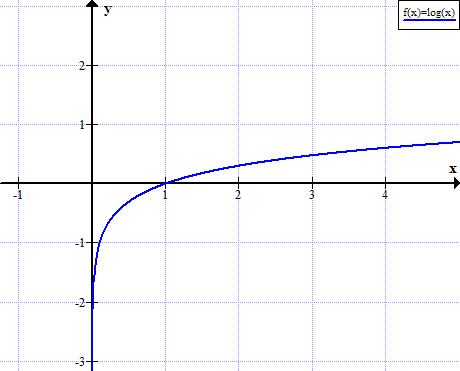
\includegraphics[width=\textwidth, height= 5.5 cm]{log_graph.png}
    \end{minipage}
    \begin{minipage}{0.9\textwidth}
    \begin{itemize}
      \item The log of a product is the sum of the logs
      \item The sum of the logs is the log of the products
      \item The log of a quotient is the difference of the logs
      \item The difference of the logs is the log of the quotient
      \item The exponent on the argument is the coefficient of the log
      \item The coefficient of the log is the exponent on the argument
    \end{itemize}
    \end{minipage}
    
\clearpage
    
\section{Problem 2}
\subsection{Requirements}
\subsection*{Requirement : 1}
    
    \begin{itemize}
      \item \textbf{ID  : } FUNR1
      \item \textbf{TYPE  : } Functional Requirement
      \item \textbf{PRIORITY  : } 1
      \item \textbf{VERSION  : } 1.0
      \item\textbf{DIFFICULTY  :} Easy
      \item \textbf{DESCRIPTION  : } System shall take two input x and base b and gives base-b logarithm of x. For example, user gives input $x= 10$ and $b = e$ then output will be 1. 
      \item\textbf{RATIONALE  : } To perform functionality on them.
      \end{itemize}
      
\subsection*{Requirement : 2}
     \begin{itemize}
      \item \textbf{ID  : } FUNR2
      \item \textbf{TYPE  : } Functional Requirement
      \item \textbf{PRIORITY  : } 1
      \item \textbf{VERSION  : } 1.0
      \item\textbf{DIFFICULTY  :} Easy
      \item \textbf{DESCRIPTION  : } When user gives negative value or zero as input to x in function $log_b x$, the system shall give the alert message that the result is not possible with this value and it should be within its domain.
      \item\textbf{RATIONALE  : } To handle the cases where input is not from its domain.
    \end{itemize}
    
\subsection*{Requirement : 3}
     \begin{itemize}
      \item \textbf{ID  : } FUNR3
      \item \textbf{TYPE  : } Functional Requirement
      \item \textbf{PRIORITY  : } 1
      \item \textbf{VERSION  : } 1.0
      \item\textbf{DIFFICULTY  :} Easy
      \item \textbf{DESCRIPTION  : } When any user gives value less than 2 as input to base b in function $log_b x$, the system shall give the alert message that the result is not possible with this value as function is defined for only base $b\neq1$ and $b>0$.
      \item\textbf{RATIONALE  : } To define the scope of the base b.
    \end{itemize}
    
\subsection*{Requirement : 4}
     \begin{itemize}
      \item \textbf{ID  : } FUNR4
      \item \textbf{TYPE  : } Functional Requirement
      \item \textbf{PRIORITY  : } 1
      \item \textbf{VERSION  : } 1.0
      \item\textbf{DIFFICULTY  :} Easy
      \item \textbf{DESCRIPTION  : } When user gives any other data type other than numbers such as string etc. as an input, the system shall not accept that type and show that input type is not properly defined.
      \item\textbf{RATIONALE  : } To define that input must be numbers.
    \end{itemize}
    
\subsection*{Requirement : 5}
     \begin{itemize}
      \item \textbf{ID  : } FUNR5
      \item \textbf{TYPE  : } Functional Requirement
      \item \textbf{PRIORITY  : } 1
      \item \textbf{VERSION  : } 1.0
      \item\textbf{DIFFICULTY  :} Easy
      \item \textbf{DESCRIPTION  : } When user gives irrational number such as e as input to base b then system shall calculate natural logarithm.
      \item\textbf{RATIONALE  : } To define natural logarithm.
    \end{itemize}
 
 
 \subsection*{Requirement : 6}
     \begin{itemize}
      \item \textbf{ID  : } NFUNR1
      \item \textbf{TYPE  : } Non-functional Requirement
      \item \textbf{PRIORITY  : } 1
      \item \textbf{VERSION  : } 1.0
      \item\textbf{DIFFICULTY  :} Easy
      \item \textbf{DESCRIPTION  : } The final output shall have some accuracy up to some point.
      \item\textbf{RATIONALE  : } To achieve proper accuracy for the system.
    \end{itemize}

\subsection*{Requirement : 7}
     \begin{itemize}
      \item \textbf{ID  : } NFUNR2
      \item \textbf{TYPE  : } Non-functional Requirement
      \item \textbf{PRIORITY  : } 1
      \item \textbf{VERSION  : } 1.0
      \item\textbf{DIFFICULTY  :} Easy
      \item \textbf{DESCRIPTION  : } The system shall respond in few seconds. 
      \item\textbf{RATIONALE  : } To achieve response time and performance speed.
    \end{itemize}  
\section{Problem 3}

\subsection{Algorithm 1 }\\
\newline
\noindent The logarithm of a given number x is the exponent to which another fixed number, the base b, must be raised, to produce that number x as the logarithm is the inverse function to exponentiation. There are many different ways to implement logarithm functions such as using Maclaurin's Series, recursion method etc. \\
The Maclaurin's Series is represented as,\\

$f(x)= f(0) +\frac{f'(0)}{1!} x +\frac{f''(0)}{2!} x^2+\frac{f'''(0)}{3!} x^3+ .....$\\

\noindent
as our function is $f(x) = log_b x$ is calculated using $\frac{\ln x}{\ln b}$, but Maclaurin's series cannot be used to find a series for $\ln x$. So, we use $\ln (l + x)$, which produces finite values for successive derivatives when $x = 0$. \\
\noindent
\newline
$f(x) = \ln (1+x)$       \\ 
$f'(x) =  \frac{1}{1+x}$\\
$f''(x) = -\frac{1}{(1+x)^2}$\\
$f'''(x) = \frac{2}{(1+x)^3}$\\

\noindent we have $f(0) = 0, f'(0) = 1, f''(0) = -1, f'''(0) = 2$ and Putting all these values in equation, we get\\

$\ln (1+x) = x - \frac{x^2}{2} + \frac{x^3}{3} - \frac{x^4}{4} ....$\hfill(1)\\

\noindent Similarly, modified logarithm series can be represented as,\\

$\ln (1-x) = - x - \frac{x^2}{2} - \frac{x^3}{3} - \frac{x^4}{4} ....$\hfill(2)\\

Instead of Considering above equations, it is better to consider their difference (1)-(2) for obtaining a better convergence.\\

$\ln (\frac{1+x}{1-x}) = 2(x + \frac{x^3}{3} + \frac{x^5}{5} + ....)$\hfill(3)\\

from (3), $\ln x = 2[(\frac{x-1}{x+1}) + \frac{1}{3}(\frac{x-1}{x+1})^3 + \frac{1}{5}(\frac{x-1}{x+1})^5 + ....]$ \\

In general, $\ln x = 2\sum_{k=1}^{\infty} \frac{1}{2k-1} (\frac{x-1}{x+1})^{2k-1}$ \\

So, $log_b x$ an be implemented as $\frac{\ln x}{\ln b}$.\\
\noindent

\noindent
The Pseudo Code for Calculating Logarithm function using series expansion is shown below.

\begin{algorithm}

\caption{Pseudo Code for Calculating Logarithm Function}

\textbf{Require:}  value: $x > 0$ And base: $b \neq 1 \vee b > 0$   \hfill //where $x,b \in \mathcal{R}^+$\\
\textbf{Ensure:} $result = \log_b x$
\begin{algorithmic}[1]

\Function {CalculatePower}{$base$, $exponent$}
    \State $power \leftarrow 1$
    
    \For {$i \leftarrow 1, exponent$}
    \State $power \leftarrow power * base$
    \EndFor
    \State \textbf{return} $power$\hfill //It returns the base to the power exponent
    \EndFunction
\Statex

\Procedure {CalculateNaturalLog}{$value$}
    \State $sum \leftarrow 0$
    \State $j \leftarrow (value-1) / (value+1)$
    \For {$i \leftarrow 1, \infty$}
    \State $k \leftarrow (2 * i) -1$
    \State $sum \leftarrow sum + (1/k) * \Call{CalculatePower}{j,k} $
    \EndFor
    \State \textbf{return} $2*sum$\hfill//It returns ln using series expansion.
    \EndProcedure
\Statex

\State $ a \leftarrow \Call{CalculateNaturalLog}{x}$\Comment{Calculates $ln x$}
\State $ b \leftarrow \Call{CalculateNaturalLog}{b}$\Comment{Calculates $ln b$}
\State $result \leftarrow a/b $\hfill //Final result of $log_b x$

\end{algorithmic}
\end{algorithm}
\subsection*{Advantages}
\begin{itemize}
    \item This form of series representation is Predictable and also it is easier to implement in programming aspect.
    \item This series is very useful for derivations
    \item It can be used to get theoretical error bounds.
\end{itemize}

\subsection*{Disadvantages}
\begin{itemize}
    \item Successive terms get very complex and hard to derive.
    \item Truncation error tends to grow rapidly away from expansion point
\end{itemize}


\subsection{Algorithm 2 }\\
\noindent The another method of implementing logarithm function is using recursion which calculates log of value x to the base b.

\noindent
The Pseudo Code for Calculating Logarithm function using simple recursion is shown below. 

\begin{algorithm}

\caption{Pseudo Code for Calculating Logarithm Function}

\textbf{Require:}  value: $x > 0$ And base: $b \neq 1 \vee b > 0$ \Comment{where $x,b \in \mathcal{R}^+$}\\
\textbf{Ensure:} $result = \log_b x$\hfill // Output will be integers.
\begin{algorithmic}[1]

\Function {CalculateLog}{$value$, $base$}
    \If {$value >base-1$}
    \State \textbf{return} $ 1 + \Call{CalculateLog}{value/base,base}$\hfill //Recursive Call
    \Else
    \State \textbf{return} $0$
    \EndIf
\EndFunction
\Statex

\State $ result \leftarrow \Call{CalculateLog}{x,,b}$\hfill // Final result of $log_b x$

\end{algorithmic}
\end{algorithm}

\subsection*{Advantages}
\begin{itemize}
    \item Complex code can be written easily in less code with Recursive method. 
\end{itemize}
\\
\newline
\subsection*{Disadvatages}
\begin{itemize}
    \item result is showing integer numbers only not any floating point.
    \item Recursive code is difficult to understand and debug.
    \item Terminating condition is must, otherwise it will go in infinite loop
    \item Execution speed decreases because of function call and return activity.
\end{itemize}

\clearpage
\begin{thebibliography}{9}
\bibitem{wiki}
\url{https://en.wikipedia.org/wiki/Logarithm}
\bibitem{rapidtables}
\url{https://www.rapidtables.com/math/algebra/Logarithm.html}
\end{thebibliography}
\end{document}

